%%%%%%%%%%%%%%%%%%%%%%%%%%%%%%%%%%%%%%%%%%%%%%%%%%%%%%%%%%%%%%%%%%%%%%%%%%%%%%%%
% LaTeX Beamer Presentation: A Survey of North American Quantum Hardware Research
% Author: Onri Jay Benally
% Date: July 27, 2025
% Scope: 10-Year Master's & PhD Output (2015-2024 Audit)
%
% INSTRUCTIONS FOR OVERLEAF:
% 1. In the Overleaf Menu (top left), go to Settings and set the "Compiler" to "XeLaTeX" or "LuaLaTeX".
% 2. Click "Recompile".
%
%%%%%%%%%%%%%%%%%%%%%%%%%%%%%%%%%%%%%%%%%%%%%%%%%%%%%%%%%%%%%%%%%%%%%%%%%%%%%%%%

\documentclass[aspectratio=169]{beamer}

%------------------------------------------------
%   PRESENTATION METADATA
%------------------------------------------------
\title[Quantum Hardware Academic Landscape]{Mapping the Quantum Hardware Academic Landscape}
\subtitle{A 10-Year Audit of Master's \& PhD Output in the U.S. and Canada (2015-2024)}
\author{Onri Jay Benally}
\institute{University of Minnesota–Twin Cities}
\date{July 27, 2025}

%------------------------------------------------
%   THEME AND STYLING
%------------------------------------------------
\usetheme{Madrid}
\usecolortheme{default}

%------------------------------------------------
%   PACKAGES
%------------------------------------------------
\usepackage{fontspec}
\usepackage{booktabs}
\usepackage{tabularx}
\usepackage{pgfplots}
\pgfplotsset{compat=1.18}
\usepackage{ragged2e}
\usepackage{siunitx} % For aligning numbers in tables
\usepackage{hyperref}
\usepackage{pifont} % For checkmarks/x-marks if needed

%------------------------------------------------
%   FONT CONFIGURATION (IBM PLEX SANS)
%------------------------------------------------
\setsansfont{IBM Plex Sans}[
  Scale=MatchLowercase,
  Ligatures=TeX,
  UprightFont = *-Regular,
  ItalicFont = *-Italic,
  BoldFont = *-SemiBold
]
\renewcommand\familydefault{\sfdefault}

%------------------------------------------------
%   FONT SIZE CONFIGURATION
%------------------------------------------------
\setbeamerfont{title}{size=\huge, series=\bfseries}
\setbeamerfont{subtitle}{size=\large}
\setbeamerfont{author}{size=\large}
\setbeamerfont{institute}{size=\normalsize}
\setbeamerfont{frametitle}{size=\Large, series=\bfseries}
\setbeamerfont{normal text}{size=\normalsize}
\setbeamerfont{block title}{size=\large}
\setbeamerfont{block body}{size=\normalsize}
\setbeamerfont{footnote}{size=\tiny}

% Custom command for table text
\newcommand{\tabletext}{\small}

%------------------------------------------------
%   PRESENTATION BEGINS
%------------------------------------------------
\begin{document}

%------------------------------------------------
% SLIDE 1: TITLE SLIDE
%------------------------------------------------
\begin{frame}
    \titlepage
\end{frame}
\note{
    Good morning. Today, I'll present a newly audited "Mapping of the Quantum Hardware Academic Landscape." This is based on a rigorous 10-year count of Master's and PhD dissertations from 2015 to 2024, giving us a much clearer picture of talent generation in the U.S. and Canada.
}

%------------------------------------------------
% SLIDE 2: INTRODUCTION (Part 1)
%------------------------------------------------
\begin{frame}
    \frametitle{Introduction:  Why Track the Full Talent Pipeline?}
    An audited count of hands-on hardware dissertations provides a more accurate view of the academic pipeline for building the quantum future.
    
    \begin{columns}[T]
        \begin{column}{0.5\textwidth}
            \begin{block}{A Tighter Focus Reveals:}
                \begin{itemize}
                    \item The true output of graduates with demonstrable hardware-building experience.
                    \item A more realistic baseline for tracking growth and assessing capacity.
                    \item The key institutions and labs driving physical quantum innovation.
                \end{itemize}
            \end{block}
        \end{column}
    \end{columns}
\end{frame}
\note{
    Why this deep audit? Because there's a difference between a theoretical thesis and one that proves a student has built or tested real hardware. This new data gives us a ground-truth measurement of the talent pool with the hands-on skills the quantum industry is built on. It shows that while earlier estimates were too high, the actual output is still impressive.
}
%------------------------------------------------
% SLIDE 3: INTRODUCTION (Part 2)
%------------------------------------------------
\begin{frame}
    \frametitle{Introduction:  Why Track the Full Talent Pipeline?}
    An audited count of hands-on hardware dissertations provides a more accurate view of the academic pipeline for building the quantum future.
    
    \begin{columns}[T]
        \begin{column}{0.5\textwidth}
            \begin{block}{A Tighter Focus Reveals:}
                \begin{itemize}
                    \item The true output of graduates with demonstrable hardware-building experience.
                    \item A more realistic baseline for tracking growth and assessing capacity.
                    \item The key institutions and labs driving physical quantum innovation.
                \end{itemize}
            \end{block}
        \end{column}
        \begin{column}{0.5\textwidth}
            \begin{block}{This Data Informs:}
                \begin{itemize}
                    \item Industry recruitment for hands-on engineering and R\&D roles.
                    \item Student choices for labs with a strong track record of hardware projects.
                    \item Policy decisions on funding for experimental research infrastructure.
                \end{itemize}
            \end{block}
        \end{column}
    \end{columns}
    \vspace{1em}        
        Quantum Hardware Lab: Group led by a principal investigator whose primary focus aligns with our hardware criteria.
\end{frame}
%------------------------------------------------
% SLIDE 3: METHODOLOGY I: SCOPE
%------------------------------------------------
\begin{frame}
    \frametitle{Methodology I: Included Hardware Categories}
    \begin{columns}[T]
        \begin{column}{0.5\textwidth}
            \begin{block}{Quantum-Core Hardware Examples}
                \begin{itemize}
                    \item \textbf{Qubit Technologies:} Superconducting (Transmon, Fluxonium), Spin-Based (NV Centers, Si/SiGe, donors, merons)
                    \item \textbf{Quantum Interconnects:} 3D Superconducting Cavities, Metamaterial/ Photonic Waveguides
                    \item \textbf{Quantum Detectors:} Superconducting Nanowire Detectors (SNSPDs), Microwave Kinetic‑Inductance Detectors (MKIDs)
                    \item \textbf{Quantum Memories:} Rare-earth doped crystals, Magnon-based devices
                \end{itemize}
            \end{block}
        \end{column}
        \begin{column}{0.5\textwidth}
            \begin{block}{Quantum-Adjacent Hardware Examples}
                \begin{itemize}
                    \item \textbf{Cryogenic Logic:} Single-Flux-Quantum (SFQ) circuits, Cryo-CMOS
                    \item \textbf{Cryogenic Mixed-Signal/RF:} DAC/ADCs, \break RF Transceiver SoCs
                    \item \textbf{Cryogenic Amplifiers:} Josephson Traveling Wave Parametric Amps (JTWPAs), HEMT LNAs
                    \item \textbf{Cryogenic Memory:} Cryo-SRAM, Cryo-MRAM, Josephson Junction-based RAM
                    \item \textbf{Cryogenic Passive Components:} On-Chip MW/RF Isolators \& Circulators
                \end{itemize}
            \end{block}
        \end{column}
    \end{columns}
\end{frame}
\note{
    At a high level, this means we counted everything from the qubits themselves to the specialized cryogenic electronics required to make them work. This provides a holistic view of the talent pool for building a complete quantum computing stack.
}
%------------------------------------------------
% SLIDE 4: METHODOLOGY II: DATA SOURCING
%------------------------------------------------
\begin{frame}
    \frametitle{Methodology II: The Audit Process}
    A multi-source audit was conducted to create a comprehensive and de-duplicated dataset for the 2015-2024 period.
    
    \begin{block}{1. Data Aggregation}
        The search pool combined three major sources:
        \begin{itemize}
            \item Institutional repositories (e.g., DSpace, EliScholar, UWSpace)
            \item ProQuest Dissertations \& Theses Global keyword exports
            \item Public lab websites ("Alumni" or "Theses" pages)
        \end{itemize}
    \end{block}
    
    \begin{block}{2. De-duplication and Normalization}
        \begin{itemize}
            \item Duplicates were removed by matching author names and ORCID iDs.
            \item Total counts were divided by ten years and rounded to the nearest 0.5.
            \item Embargoed theses (~10\%) were estimated from public defense announcements.
        \end{itemize}
    \end{block}
\end{frame}
\note{
    Our process was meticulous. We aggregated data from university libraries, the ProQuest database, and individual lab websites. We then carefully de-duplicated the entries to ensure each thesis was counted only once. Finally, we normalized the data to get the average annual output. This rigorous process gives us higher confidence in the final numbers.
}

%------------------------------------------------
% SLIDE 5: A FOUR-TIER SYSTEM
%------------------------------------------------
\begin{frame}
    \frametitle{A Four-Tier System}
    Based on the 10-year audited data, universities have been grouped into four tiers reflecting their scale of combined Master's and PhD production.
    
    \begin{center}
    \begin{tabularx}{0.9\textwidth}{l >{\RaggedRight}X}
        \toprule
        \textbf{Tier} & \textbf{Description (Avg. Total Theses/ Year)} \\
        \midrule
        \textbf{Tier 1: High-volume producers} & Institutions with large, sustained output ($\geq 5$). \\
        \addlinespace
        \textbf{Tier 2: Moderate producers} & Universities with strong, consistent output ($3 - 4.9$). \\
        \addlinespace
        \textbf{Tier 3: Niche producers} & Universities with established, focused programs \break ($1.5 - 2.9$). \\
        \addlinespace
        \textbf{Tier 4: Emerging nodes} & Institutions with smaller or developing programs \break ($< 1.5$). \\
        \bottomrule
    \end{tabularx}
    \end{center}
    Note: Data on lab counts is approximate.
\end{frame}
\note{
    To organize the data, we've used a four-tier system. A Tier 1 "High-volume producer" is an institution averaging five or more hardware theses per year. This classification helps to meaningfully distinguish the scale and concentration of hands-on research training across North America.
}

%------------------------------------------------
% SLIDE 6: TIER 1 - HIGH-VOLUME PRODUCERS
%------------------------------------------------
\begin{frame}
    \frametitle{Tier 1: The Research Powerhouses}
    High-volume producers with $\geq 5$ total theses per year
    \begin{table}
        \centering
        \tabletext
        \begin{tabularx}{\textwidth}{
            l
            S[table-format=1.1]
            S[table-format=2.0, table-space-text-pre=~]
        }
            \toprule
            \textbf{University} & {\textbf{Theses/yr}} & {\textbf{Labs}} \\
            \midrule
            Yale University & 6.0 & ~6 \\
            U. of Maryland, College Park (JQI) & 5.5 & ~10 \\
            Massachusetts Institute of Technology (MIT) & 5.0 & ~14 \\
            \bottomrule
        \end{tabularx}
    \end{table}
    
    \begin{block}{Key Takeaway}
    A highly elite group of three universities forms the top tier, acting as the primary engines for training the next generation of quantum hardware leaders.
    \end{block}
\end{frame}
\note{
    Our audit reveals a very concentrated top tier. Yale, the University of Maryland, and MIT are in a class of their own, each producing a significant volume of hands-on hardware theses year after year. These three institutions are the current epicenters of hardware-focused talent production.
}

%------------------------------------------------
% SLIDE 7: TIER 2 - MODERATE PRODUCERS
%------------------------------------------------
\begin{frame}
    \frametitle{Tier 2: The Core of Innovation}
    Moderate producers with 3 - 4.9 total theses per year
    
    \begin{table}
        \centering
        \tabletext
        \begin{tabularx}{\textwidth}{
            l
            S[table-format=1.1]
            S[table-format=2.0, table-space-text-pre=~]
        }
            \toprule
            \textbf{University} & {\textbf{Theses/yr}} & {\textbf{Labs}} \\
            \midrule
            UC Berkeley & 4.5 & ~8 \\
            U. of Waterloo (IQC) & 4.0 & ~24 \\
            Princeton University & 4.0 & ~5 \\
            UC Santa Barbara & 4.0 & ~4 \\
            Harvard University & 3.5 & ~7 \\
            Stanford University & 3.5 & ~6 \\
            U. of Wisconsin-Madison & 3.5 & ~4 \\
            U. of Chicago & 3.0 & ~6 \\
            Caltech & 3.0 & ~5 \\
            \bottomrule
        \end{tabularx}
    \end{table}
\end{frame}
\note{
    Tier 2 comprises the major research universities that are critical to the health of the quantum ecosystem. While not at the same volume as Tier 1, institutions like Berkeley, Waterloo, and Princeton are producing a substantial and steady number of hardware-focused graduates.
}

%------------------------------------------------
% SLIDE 8: ANALYSIS: THE PRODUCTION CADENCE
%------------------------------------------------
\begin{frame}
    \frametitle{Analysis: The Production Cadence}
    \begin{center}
        \begin{tikzpicture}
            \begin{axis}[
                xbar,
                width=0.9\textwidth,
                height=0.75\textheight,
                bar width=9pt,
                enlarge y limits={0.1},
                xlabel={Avg. Annual Quantum-Hardware-Related Theses Output},
                xmin=0,
                xmax=6.5,
                % The order here dictates the order on the y-axis, from bottom to top.
                symbolic y coords={
                    UChicago,
                    Caltech,
                    UW-Madison,
                    Stanford,
                    Harvard,
                    Princeton,
                    Waterloo,
                    UCSB,
                    UCBerkeley,
                    MIT,
                    Maryland,
                    Yale
                },
                ytick=data,
                yticklabel style={font=\small, align=right},
                nodes near coords,
                nodes near coords style={font=\small},
                nodes near coords align={horizontal},
            ]
            % The data must be in the same order as the symbolic y coords.
            \addplot coordinates {
                (3.0,UChicago)
                (3.0,Caltech)
                (3.5,UW-Madison)
                (3.5,Stanford)
                (3.5,Harvard)
                (4.0,Princeton)
                (4.0,Waterloo)
                (4.0,UCSB)
                (4.5,UCBerkeley)
                (5.0,MIT)
                (5.5,Maryland)
                (6.0,Yale)
            };
            \end{axis}
        \end{tikzpicture}
    \end{center}
    Collectively, Yale, UMD, and MIT lead at roughly one quantum-hardware-related thesis every two months. The nine schools in Tier 2 deliver one every three to four months. 
\end{frame}
\note{
    This chart visualizes the output of the top 12 universities. What this means in practical terms is that the Tier 1 schools graduate a student with hands-on hardware experience about every two months. The Tier 2 schools are on a cadence of about one every quarter. This highlights a significant concentration of talent generation at the very top.
}

%------------------------------------------------
% SLIDE 9: TIER 3 - NICHE PRODUCERS (PART 1)
%------------------------------------------------
\begin{frame}
    \frametitle{Tier 3: The Diverse Research Ecosystem (Part 1)}
    Niche producers with 1.5 - 2.9 total theses per year
    
    \begin{table}
        \centering
        \tabletext
        \begin{tabularx}{\textwidth}{
            l
            S[table-format=1.1]
            S[table-format=2.0, table-space-text-pre=~]
        }
            \toprule
            \textbf{University} & {\textbf{Theses/yr}} & {\textbf{Labs}} \\
            \midrule
            U. of British Columbia (QMI) & 2.5 & ~12 \\
            U. of Toronto (CQIQC) & 2.5 & ~10 \\
            U. of Colorado Boulder (JILA) & 2.5 & ~6 \\
            U. de Sherbrooke (IQ) & 2.0 & ~11 \\
            U. of Michigan & 2.0 & ~4 \\
            Duke University & 2.0 & ~4 \\
            U. of Texas at Austin & 2.0 & ~4 \\
            Cornell University & 2.0 & ~4 \\
            \bottomrule
        \end{tabularx}
    \end{table}
\end{frame}
\note{
    Moving to Tier 3, we find a broad and vital group of universities with established, specialized programs. Institutions like UBC, Toronto, and CU Boulder are significant hubs of expertise, contributing a steady stream of researchers with focused skill sets, typically at a rate of a few theses per year.
}

%------------------------------------------------
% SLIDE 10: TIER 3 - NICHE PRODUCERS (PART 2)
%------------------------------------------------
\begin{frame}
    \frametitle{Tier 3: The Diverse Research Ecosystem (Part 2)}
    Niche producers with 1.5 - 2.9 total theses per year
    
    \begin{table}
        \centering
        \tabletext
        \begin{tabularx}{\textwidth}{
            l
            S[table-format=1.1]
            S[table-format=2.0, table-space-text-pre=~]
        }
            \toprule
            \textbf{University} & {\textbf{Theses/yr}} & {\textbf{Labs}} \\
            \midrule
            McGill University & 1.5 & ~6 \\
            U. of Calgary & 1.5 & ~5 \\
            U. of Alberta & 1.5 & ~5 \\
            Rice University & 1.5 & ~3 \\
            Penn State University & 1.5 & ~3 \\
            Northwestern U. & 1.5 & ~3 \\
            Georgia Tech & 1.5 & ~3 \\
            UCLA & 1.5 & ~3 \\
            UC San Diego & 1.5 & ~3 \\
            UIUC & 1.5 & ~3 \\
            U. of Washington & 1.5 & ~3 \\
            \bottomrule
        \end{tabularx}
    \end{table}
\end{frame}
\note{
    Here is the second half of our extensive Tier 3 list. The key story of this tier is its breadth and depth. These universities ensure that quantum talent and specialized knowledge are being developed across the continent, fostering a more resilient and diverse national research enterprise.
}

%------------------------------------------------
% SLIDE 11: TIER 4 - EMERGING NODES
%------------------------------------------------
\begin{frame}
    \frametitle{Tier 4: Emerging Nodes}
    Producers with $<$ 1.5 total theses per year, representing growth potential
    
    \begin{table}
        \centering
        \tabletext
        \begin{tabularx}{\textwidth}{
            l
            S[table-format=1.1]
            S[table-format=2.0, table-space-text-pre=~]
        }
            \toprule
            \textbf{University} & {\textbf{Theses/yr}} & {\textbf{Labs}} \\
            \midrule
            U. of Minnesota-TC & 1.0 & ~5 \\
            Simon Fraser U. & 1.0 & ~4 \\
            Columbia University & 1.0 & ~3 \\
            U. de Montréal & 1.0 & ~3 \\
            Arizona State U. & 1.0 & ~3 \\
            U. of Pittsburgh & 1.0 & ~3 \\
            UC Davis & 1.0 & ~2 \\
            U. of New Mexico & 1.0 & ~2 \\
            U. of Rochester & 1.0 & ~2 \\
            U. of Arizona & 1.0 & ~2 \\
            Université Laval & 1.0 & ~2 \\
            U. of Victoria & 0.5 & ~2 \\
            \bottomrule
        \end{tabularx}
    \end{table}
\end{frame}
\note{
    Finally, Tier 4. These emerging nodes are essential for niche expertise and regional talent development. While their output is smaller—typically one thesis per year or less—they are the training grounds for future specialists and represent the potential for growth in the academic landscape.
}

%------------------------------------------------
% SLIDE 12: GEOGRAPHIC VIEW I: U.S. HUBS
%------------------------------------------------
\begin{frame}
    \frametitle{Geographic View I: Major U.S. Hubs}
    Hardware talent production in the United States is concentrated in three major geographic clusters.
    
    \begin{block}{Northeast Corridor}
        A dense cluster of talent production from Boston (MIT, Harvard) and New Haven (Yale) down to Maryland (JQI) and Princeton. This is the most productive region in North America.
    \end{block}
    
    \begin{block}{California}
        A bi-modal hub with major centers in the Bay Area (Stanford, Berkeley) and Southern California (Caltech, UCSB, UCLA, UCSD).
    \end{block}
    
    \begin{block}{Midwest Hub}
        A strong regional cluster anchored by the University of Chicago, University of Wisconsin, and UIUC, forming a core of talent in the nation's interior.
    \end{block}
\end{frame}
\note{
    When we look at the geography of talent, the US shows three dominant hubs. The Northeast Corridor is the most dense and productive. California is a close second, with two major centers of gravity. And the Midwest Hub is a critical center of research in the middle of the country.
}

%------------------------------------------------
% SLIDE 13: GEOGRAPHIC VIEW II: THE CANADIAN CORRIDOR
%------------------------------------------------
\begin{frame}
    \frametitle{Geographic View II: The Canadian Quantum Corridor}
    Canada's institute-driven model has created a powerful, distributed ecosystem.

    \begin{table}
        \centering
        \tabletext
        \begin{tabularx}{\textwidth}{
            l
            S[table-format=1.1]
        }
            \toprule
            \textbf{University} & {\textbf{Theses/yr}} \\
            \midrule
            U. of Waterloo (IQC) & 4.0 \\
            U. of British Columbia (QMI) & 2.5 \\
            U. of Toronto (CQIQC) & 2.5 \\
            U. de Sherbrooke (IQ) & 2.0 \\
            U. of Calgary / U. of Alberta / McGill & 1.5 \\
            \bottomrule
        \end{tabularx}
    \end{table}
    \begin{block}{Observation}
    From the Ontario-Québec axis (Waterloo, Toronto, Sherbrooke) to the strong Western presence (UBC, Calgary, Alberta), Canadian universities are prominent in Tiers 2 and 3, often anchored by dedicated quantum institutes.
    \end{block}
\end{frame}
\note{
    Canada's strategy has been different, focusing on building large, dedicated institutes. This has paid off, creating a powerful corridor of talent. Waterloo is the anchor, but the ecosystem is strong from coast to coast, with major centers in BC, Alberta, Ontario, and Quebec.
}

%------------------------------------------------
% SLIDE 14: KEY FINDING I: CONCENTRATION AT THE TOP
%------------------------------------------------
\begin{frame}
    \frametitle{Key Finding I: Extreme Concentration at the Top}
    
    \begin{alertblock}{The Takeaway}
        The production of hands-on quantum hardware talent is dominated by a very small number of elite institutions.
    \end{alertblock}
    
    \begin{itemize}
        \item The top 3 universities (Yale, UMD, MIT) collectively produce \textbf{16.5 theses/year}, accounting for a significant fraction of the total output of all listed schools.
        \item The top 12 universities (Tiers 1 \& 2) collectively produce \textbf{45 theses/year}, representing the vast majority of the talent pipeline.
        \item This concentration has significant implications for recruitment, collaboration, and the geographic distribution of the quantum industry.
    \end{itemize}
\end{frame}
\note{
    Our first major finding is the extreme concentration of talent production. The top three schools alone account for a massive portion of the total output. If you expand that to the top twelve schools in Tiers 1 and 2, you've accounted for the lion's share of the entire North American talent pipeline.
}

%------------------------------------------------
% SLIDE 15: KEY FINDING II: A MORE REALISTIC BASELINE
%------------------------------------------------
\begin{frame}
    \frametitle{Key Finding II: A More Realistic Baseline}
    
    \begin{alertblock}{The Takeaway}
        Estimates of talent output need to be carefully compiled. This audit provides a more sober, actionable baseline for the community.
    \end{alertblock}
    
    \begin{itemize}
        \item By focusing only on theses with demonstrable hardware components, we gain a clearer signal on the pipeline for builders and experimentalists.
        \item No single institution is currently producing ten or more hardware-focused theses per year.
        \item This realistic baseline is critical for accurately forecasting workforce growth and identifying true gaps in the educational pipeline.
    \end{itemize}
\end{frame}
\note{
    Our second key finding is that the real-world output of hardware-focused graduates is lower than some have estimated. By filtering out purely theoretical or software work, we arrive at a more realistic number. This is not bad news; it's better data. It gives us a solid, defensible baseline to track future growth and to make smarter investments in education.
}

%------------------------------------------------
% SLIDE 16: KEY FINDING III: THE VITAL BROADER ECOSYSTEM
%------------------------------------------------
\begin{frame}
    \frametitle{Key Finding III: The Vital Broader Ecosystem}
    
    \begin{alertblock}{The Takeaway}
        While output is concentrated, the numerous universities in Tiers 3 and 4 are essential for the long-term health and diversity of the field.
    \end{alertblock}
    
    \begin{itemize}
        \item These $\sim$30 institutions provide crucial geographic diversity, preventing over-concentration of talent in a few coastal hubs.
        \item They are hubs for specialized expertise in specific hardware modalities that may not exist at the larger schools.
        \item They represent the primary growth opportunity for expanding the North American talent pipeline in the coming decades.
    \end{itemize}
\end{frame}
\note{
    Our final key finding is about the importance of the rest of the ecosystem. While the top schools get the headlines, the dozens of universities in Tiers 3 and 4 are absolutely critical. They provide geographic balance, they are hubs of specialized knowledge, and they represent the biggest opportunity for growing the talent pool in the years ahead.
}

%------------------------------------------------
% SLIDE 17: CONCLUSION & FUTURE OUTLOOK
%------------------------------------------------
\begin{frame}
    \frametitle{Conclusion \& Future Outlook}
    The North American academic landscape for quantum hardware is robust, but the pipeline for graduates with hands-on experience is highly concentrated.
    
    \begin{block}{Future Considerations}
        \begin{itemize}
            \item Will we see more universities ascend to the top tiers as national funding initiatives mature?
            \item How does this academic output map to the founding of startups and corporate hiring patterns?
            \item A scripted, annual crawl of repositories could tighten the current error bars from $\pm$10\% to $\pm$5\%.
            \item Tracking the growth of Tier 4 "emerging nodes" will be key to identifying the next generation of leading programs.
        \end{itemize}
    \end{block}
    
\end{frame}
\note{
    In conclusion, our audit shows a productive but highly concentrated ecosystem for training quantum hardware experts. Looking forward, it will be crucial to see if this landscape becomes more distributed over time. The next phase of this research should be to automate this audit for annual updates and to directly map this academic output to innovation metrics like startup formation.
}

%------------------------------------------------
% SLIDE 18: QUESTIONS
%------------------------------------------------
\begin{frame}
    \frametitle{Thank You}
    
    \vfill
    
    \begin{center}
        \Huge \textbf{Questions?}
    \end{center}
    
    \vfill
    
\end{frame}
\note{
    Thank you for your attention. I would be happy to take your questions.
}

%------------------------------------------------
% SLIDE 19: APPENDIX I: DATA & METHODOLOGY
%------------------------------------------------
\begin{frame}[fragile]
    \frametitle{Appendix I: Audit Methodology \& Caveats}
    \begin{block}{Query Design \& De-duplication}
        We issued compound boolean searches (e.g., \texttt{\tiny("superconducting" OR "cryo-CMOS") AND "thesis"}) across 41 repositories and ProQuest for the 2015-2024 period. Duplicates were removed via ORCID/author matching. Counts were normalized to annual averages.
    \end{block}
    
    \begin{block}{Caveats \& Error Bars}
        \begin{itemize}
            \item \textbf{Hidden M.Sc. Work:} Some EE departments archive Master’s theses locally, so these numbers may be a slight under-count.
            \item \textbf{Uncertainty:} Residual uncertainty is estimated at $\pm$0.7 theses/yr for Tier 1, $\pm$0.5 for Tier 2, and $\pm$0.3 elsewhere.
        \end{itemize}
    \end{block}

    \begin{block}{Acronyms}
        \tiny \textbf{cQED:} Circuit Quantum Electrodynamics; \textbf{IQC/IQ:} Institute for Quantum Computing/Institut Quantique; \textbf{JQI/JILA:} Joint Quantum Inst./Joint Inst. for Lab. Astrophysics; \textbf{SFQ:} Single-Flux-Quantum
    \end{block}
\end{frame}

%------------------------------------------------
% SLIDE 20: APPENDIX II: RAW DATA
%------------------------------------------------
\begin{frame}[fragile]
    \frametitle{Appendix II: Audited Annual Thesis Output (2015-2024)}
    \vspace{-2mm}
    \tiny 
    \begin{columns}[T]
        \begin{column}{0.5\textwidth}
            \begin{tabularx}{\linewidth}{r @{.} l S[table-format=1.1]}
                \toprule
                \multicolumn{2}{l}{\textbf{University}} & {\textbf{Theses/yr}} \\
                \midrule
                1 & Yale University & 6.0 \\
                2 & U. of Maryland & 5.5 \\
                3 & MIT & 5.0 \\
                4 & UC Berkeley & 4.5 \\
                5 & U. of Waterloo & 4.0 \\
                6 & Princeton University & 4.0 \\
                7 & UC Santa Barbara & 4.0 \\
                8 & Harvard University & 3.5 \\
                9 & Stanford University & 3.5 \\
                10 & U. of Wisconsin-Madison & 3.5 \\
                11 & Caltech & 3.0 \\
                12 & U. of Chicago & 3.0 \\
                13 & U. of British Columbia & 2.5 \\
                14 & U. of Toronto & 2.5 \\
                15 & U. of Colorado Boulder & 2.5 \\
                16 & U. de Sherbrooke & 2.0 \\
                17 & U. of Michigan & 2.0 \\
                18 & Duke University & 2.0 \\
                19 & U. of Texas at Austin & 2.0 \\
                20 & Cornell University & 2.0 \\
                \bottomrule
            \end{tabularx}
        \end{column}
        \begin{column}{0.5\textwidth}
            \begin{tabularx}{\linewidth}{r @{.} l S[table-format=1.1]}
                \toprule
                \multicolumn{2}{l}{\textbf{University}} & {\textbf{Theses/yr}} \\
                \midrule
                21 & Rice University & 1.5 \\
                22 & Penn State University & 1.5 \\
                23 & Northwestern U. & 1.5 \\
                24 & Georgia Tech & 1.5 \\
                25 & UCLA & 1.5 \\
                26 & UC San Diego & 1.5 \\
                27 & U. of Alberta & 1.5 \\
                28 & U. of Calgary & 1.5 \\
                29 & McGill University & 1.5 \\
                30 & UIUC & 1.5 \\
                31 & U. of Washington & 1.5 \\
                32 & UC Davis & 1.0 \\
                33 & Simon Fraser U. & 1.0 \\
                34 & Columbia University & 1.0 \\
                35 & U. de Montréal & 1.0 \\
                36 & Arizona State U. & 1.0 \\
                37 & U. of New Mexico & 1.0 \\
                38 & U. of Rochester & 1.0 \\
                39 & U. of Arizona & 1.0 \\
                40 & Université Laval & 1.0 \\
                41 & U. of Minnesota-TC & 1.0 \\
                42 & U. of Pittsburgh & 1.0 \\
                43 & U. of Victoria & 0.5 \\
                \bottomrule
            \end{tabularx}
        \end{column}
    \end{columns}
\end{frame}

\end{document}
